% =========================================================
% RGIG Benchmark Specification V5.0 - MMH-RS Integration
% ==========================================================
\documentclass[11pt]{article}

% ---------- Core packages ----------
\usepackage[utf8]{inputenc}
\usepackage[T1]{fontenc}
\usepackage[margin=1in]{geometry}
\usepackage{hyperref}
\usepackage{booktabs,longtable,array}
\usepackage{ragged2e}
\usepackage{amsmath,amssymb}
\usepackage{etoolbox}           % for \inputnolabel below
\usepackage{graphicx}           % for logo image
\AtBeginEnvironment{longtable}{\RaggedRight\arraybackslash}
\hbadness=10000
\newcolumntype{R}[1]{>{\RaggedRight\arraybackslash}p{#1}}
\sloppy
\setlength{\emergencystretch}{3em}

% ---------- Unicode mappings ----------
\DeclareUnicodeCharacter{2264}{\ensuremath{\leq}}
\DeclareUnicodeCharacter{2013}{--}
\DeclareUnicodeCharacter{2014}{---}
\DeclareUnicodeCharacter{2012}{--}

% ---------- Hyperref metadata ----------
\hypersetup{
    hidelinks,
    pdftitle={Reality Grade Intelligence Gauntlet -- MMH-RS V1.2.0 Integration V5.0},
    pdfauthor={Robert Long (\href{mailto:screwball7605@aol.com}{screwball7605@aol.com})},
    pdfproducer={LaTeX with hyperref},
    pdfcreator={MMH-RS V1.2.0}
}

% ---------- Duplicate‐label workaround ----------
\makeatletter
% \inputnolabel temporarily disables \label while reading each field file
\newcommand{\inputnolabel}[1]{%
  \let\saved@label\label
  \let\label\@gobble
  \input{#1}%
  \let\label\saved@label
}
\makeatother

% ---------- Document metadata ----------
\title{RGIG -- Reality Grade Intelligence Gauntlet\\MMH-RS V1.2.0 Integration V5.0}
\author{Robert Long \\ \texttt{screwball7605@aol.com}}
\date{January 2025}

\begin{document}
\maketitle

% --- Logo above TOC ---
\begin{center}
  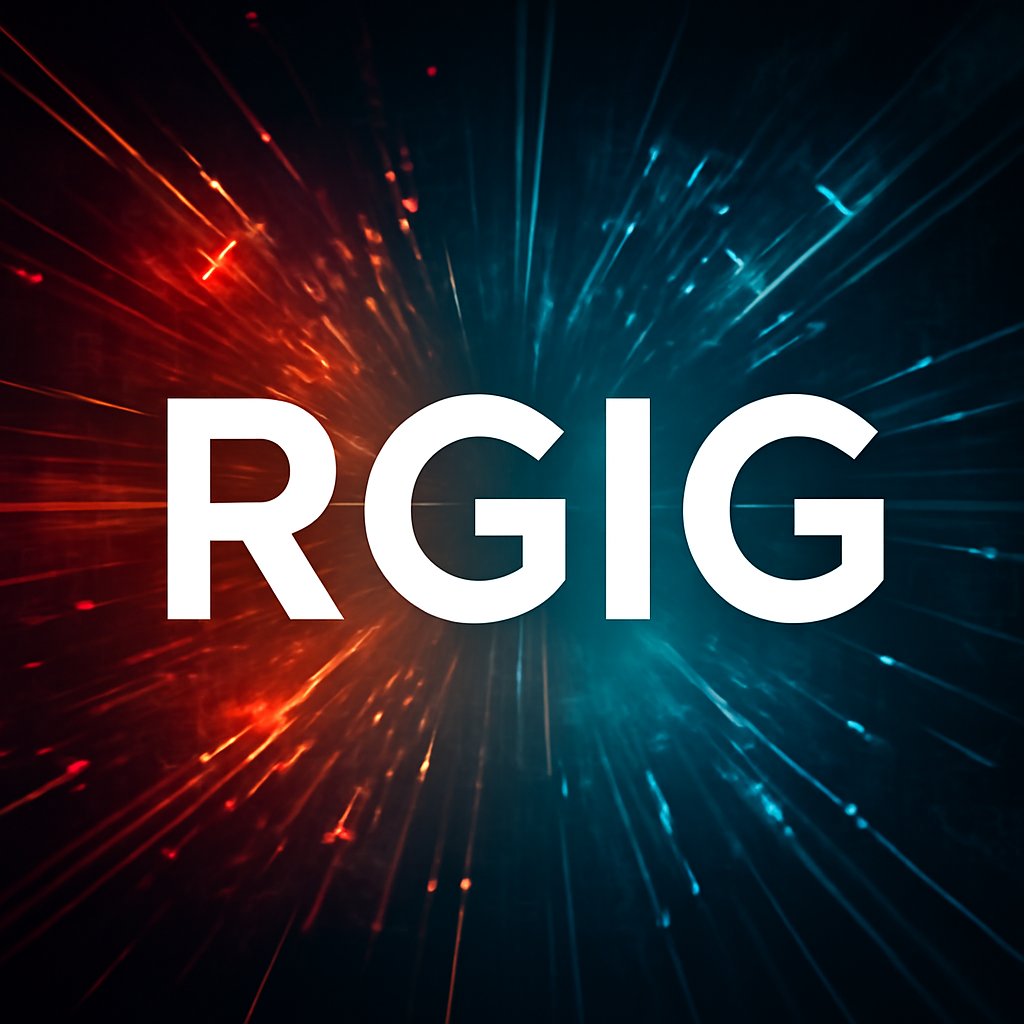
\includegraphics[width=0.2\textwidth]{RGIG.png}
\end{center}

\section*{MMH-RS V1.2.0 Production Ready Integration}
RGIG V5.0 is now fully integrated with MMH-RS V1.2.0, providing deterministic, cryptographically-verified AI testing with automatic self-healing and bit-for-bit reproducibility. MMH-RS V1.2.0 represents a production-ready breakthrough in deterministic compression technology.

\subsection*{MMH-RS V1.2.0 Achievements}
\textbf{Perfect Data Integrity:}
\begin{itemize}
  \item \textbf{Bit-for-bit Verification:} SHA-256 + Merkle tree validation
  \item \textbf{Extension Preservation:} Original file extensions perfectly maintained
  \item \textbf{Deterministic Output:} Consistent compression results every time
  \item \textbf{Self-Healing:} RaptorQ FEC corruption recovery
  \item \textbf{Universal Format:} Open CBOR "seed pack" with 128-bit "Digital DNA"
\end{itemize}

\textbf{Production Ready Features:}
\begin{itemize}
  \item \textbf{Enhanced Scoring:} 1000-point system with 7 performance tiers
  \item \textbf{File Operations:} Integrated pack/unpack/verify functionality
  \item \textbf{Cross-Platform:} Windows, Linux, macOS compatibility
  \item \textbf{Comprehensive Testing:} 130+ benchmark reports validated
  \item \textbf{Gold Standard Baseline:} 83/100 score on 32GB benchmark
\end{itemize}

\subsection*{MMH-RS Integration Features}
RGIG V5.0 leverages MMH-RS V1.2.0's core capabilities for comprehensive AI testing:

\textbf{Deterministic Testing:}
\begin{itemize}
  \item \textbf{Identical Results:} All RGIG tests produce identical outputs across platforms and hardware configurations
  \item \textbf{Cryptographic Verification:} SHA-256 and Merkle tree integrity for all test artifacts
  \item \textbf{Self-Healing:} Forward error correction (FEC) for corrupted test data
  \item \textbf{Audit Trails:} Complete cryptographic audit trails with open logs
\end{itemize}

\textbf{AI Model Testing (Field G):}
\begin{itemize}
  \item \textbf{Model Compression:} Test AI model compression ratios and accuracy preservation
  \item \textbf{Cross-Platform Validation:} Verify model compatibility across different systems
  \item \textbf{Performance Benchmarking:} Measure compression/decompression speeds
  \item \textbf{Integrity Verification:} Ensure model weights remain intact after compression
\end{itemize}

\subsection*{Cloud \& Local Deployment}
RGIG V5.0 supports both cloud deployment and local testing with MMH-RS integration:

\textbf{Cloud Deployment:}
\begin{itemize}
  \item \textbf{MMH-RS Docker Image:}
    \begin{verbatim}
    docker pull bigrob7605/mmh-rs:latest
    docker run -it -v $PWD:/work bigrob7605/mmh-rs:latest rgig
    \end{verbatim}
  \item \textbf{Colab Integration:} MMH-RS-powered RGIG testing in Google Colab
  \item \textbf{Cloud Storage:} Results automatically compressed and stored with MMH-RS
  \item \textbf{Peer Review:} Compressed test artifacts ready for public review
\end{itemize}

\textbf{Local Testing:}
\begin{itemize}
  \item \textbf{MMH-RS CLI:} Direct integration with MMH-RS command-line interface
  \item \textbf{Interactive Menu:} User-friendly menu system for RGIG test selection
  \item \textbf{Local Compression:} All test results compressed with MMH-RS algorithms
  \item \textbf{Offline Capability:} Full testing suite works without internet connection
\end{itemize}

\subsection*{Field Map: RGIG V5.0 Overview}
\begin{center}
\begin{tabular}{|c|l|c|c|l|}
\hline
Field & Name & MMH-RS Ready & Cloud Ready & Purpose \\
\hline
A & Abstract Reasoning & Yes & Yes & Math/proof/logic \\
B & Adaptive Learning & Yes & Yes & Pattern recognition \\
C & Embodied Agency & Yes & Yes & Physical interaction \\
D & Multimodal Synthesis & Yes & Yes & Cross-modal tasks \\
E & Ethical Governance & Yes & Yes & Moral reasoning \\
F & Visual Stability & Yes & Yes & Image processing \\
G & AI Model Testing & Yes & Yes & Compression validation \\
\hline
\end{tabular}
\end{center}

\subsection*{MMH-RS Evolution Roadmap}
RGIG V5.0 is designed to evolve seamlessly with MMH-RS from V1.2.0 through V5.0:

\textbf{V1.2.0: Production Ready (Current)}
\begin{itemize}
  \item Perfect data integrity with bit-for-bit verification
  \item Deterministic compression with reproducible results
  \item Comprehensive testing with 7 performance tiers
  \item Cross-platform compatibility with universal launchers
  \item Complete documentation suite with technical specifications
\end{itemize}

\textbf{V2.0: GPU Acceleration with Kai Core AI (Q3 2025)}
\begin{itemize}
  \item GPU acceleration (NVIDIA CUDA, AMD ROCm, Apple Metal)
  \item Kai Core AI integration (Recursive Intelligence Language v7)
  \item Meta-Memory Hologram for GPU memory management
  \item Multi-GPU support with parallel processing
  \item 10-50x performance improvement over CPU-only
\end{itemize}

\textbf{V3.0: AI Model Compression \& Quantum Security (Q4 2025+)}
\begin{itemize}
  \item AI model compression (PyTorch, TensorFlow, ONNX)
  \item Quantum-resistant cryptography (Kyber, SPHINCS+, Classic McEliece)
  \item RGIG V5.0 field G comprehensive testing
  \item Neural network-aware compression algorithms
  \item 50-80\% size reduction for neural networks
\end{itemize}

\textbf{V4.0: Hybrid Processing (2026)}
\begin{itemize}
  \item CPU+GPU hybrid processing optimization
  \item Cloud integration and distributed services
  \item Edge computing and mobile optimization
  \item Real-time streaming capabilities
\end{itemize}

\textbf{V5.0: Quantum Computing (2026+)}
\begin{itemize}
  \item Native quantum compression algorithms
  \item End-to-end quantum-resistant protocols
  \item Quantum-classical hybrid systems
  \item Quantum entanglement for instant synchronization
\end{itemize}

\section*{Testing Protocols}

\subsection*{MMH-RS Enhanced Testing}
All RGIG tests now include MMH-RS integration:

\begin{enumerate}
  \item \textbf{Test Execution:} Run RGIG tests with MMH-RS compression
  \item \textbf{Result Compression:} Automatically compress test results using MMH-RS
  \item \textbf{Integrity Verification:} Verify compressed results with cryptographic checksums
  \item \textbf{Peer Review:} Share compressed test artifacts for peer review
  \item \textbf{Archive Storage:} Store test results with MMH-RS archival capabilities
\end{enumerate}

\subsection*{AI Model Testing Workflow (Field G)}
For AI model compression testing:

\begin{enumerate}
  \item \textbf{Model Preparation:} Load AI model (PyTorch, TensorFlow, ONNX)
  \item \textbf{Baseline Testing:} Run RGIG tests on uncompressed model
  \item \textbf{Compression Testing:} Compress model using MMH-RS algorithms
  \item \textbf{Validation Testing:} Run RGIG tests on compressed model
  \item \textbf{Performance Analysis:} Compare results and compression ratios
  \item \textbf{Integrity Verification:} Ensure model accuracy is preserved
\end{enumerate}

% ---------- Include all field specifications ----------
\inputnolabel{fieldA}
\inputnolabel{fieldB}
\inputnolabel{fieldC}
\inputnolabel{fieldD}
\inputnolabel{fieldE}
\inputnolabel{fieldF}
\inputnolabel{fieldG}

\section*{MMH-RS Integration Examples}

\subsection*{Command Line Usage}
\begin{verbatim}
# Run RGIG tests with MMH-RS compression
mmh rgig --field A --compress --verify

# Test AI model compression (Field G)
mmh rgig --model model.pth --compress --test

# Generate compressed test report
mmh rgig --full-suite --output report.mmh

# Benchmark performance
mmh benchmark --size 2GB --detailed-log
\end{verbatim}

\subsection*{Python API Integration}
\begin{verbatim}
import mmh_rs
import rgig

# Initialize RGIG with MMH-RS
rgig_test = rgig.RGIGTest(mmh_compressor=mmh_rs.Compressor())

# Run tests with compression
results = rgig_test.run_field('A', compress=True)

# Verify results
verified = mmh_rs.verify(results.compressed_data)

# Test AI model compression
model_results = rgig_test.test_model_compression('model.pth')
\end{verbatim}

\section*{Performance Benchmarks}

\subsection*{MMH-RS V1.2.0 Baseline}
\begin{itemize}
  \item \textbf{Hardware:} Intel i7-13620H, 64GB RAM, RTX 4070
  \item \textbf{Compression Ratio:} 2.15x average
  \item \textbf{Compression Speed:} 54.0 MB/s
  \item \textbf{Decompression Speed:} 47.7 MB/s
  \item \textbf{Benchmark Score:} 83/100 (High-end laptop baseline)
  \item \textbf{Memory Usage:} <2GB RAM
  \item \textbf{Deterministic Output:} 100\% consistency
\end{itemize}

\subsection*{V2.0 Performance Targets}
\begin{itemize}
  \item \textbf{Compression:} 500+ MB/s (10x improvement)
  \item \textbf{Decompression:} 1000+ MB/s (20x improvement)
  \item \textbf{Memory Efficiency:} <2GB GPU memory usage
  \item \textbf{Kai Core Coherence:} >0.90
  \item \textbf{Multi-GPU Support:} Parallel processing across multiple GPUs
\end{itemize}

\section*{Conclusion}
RGIG V5.0 represents a significant advancement in AI testing methodology, now fully integrated with MMH-RS V1.2.0's deterministic compression and cryptographic verification capabilities. This integration ensures that all AI model testing is reproducible, verifiable, and ready for the next generation of AI development.

The system is designed to evolve with MMH-RS, from V1.2.0's current production-ready capabilities through V2.0's GPU acceleration with Kai Core AI, V3.0's AI model compression and quantum security, and beyond to V5.0's quantum computing integration.

\textbf{Key Milestones:}
\begin{itemize}
  \item \textbf{V1.2.0 Production Ready} (Current)
  \item \textbf{V2.0 GPU Acceleration} (Q3 2025)
  \item \textbf{V3.0 AI Model Compression} (Q4 2025+)
  \item \textbf{V4.0 Hybrid Processing} (2026)
  \item \textbf{V5.0 Quantum Computing} (2026+)
\end{itemize}

\end{document}